%%%%%%%%%%%%%%%%%%%%%%%%%%%%%%%%%%%%%%%%%%%%%%%%%%%%%%%%%%%
% --------------------------------------------------------
% Tau
% LaTeX Template
% Version 2.4.4 (28/02/2025)
%
% Author: 
% Guillermo Jimenez (memo.notess1@gmail.com)
% 
% License:
% Creative Commons CC BY 4.0
% --------------------------------------------------------
%%%%%%%%%%%%%%%%%%%%%%%%%%%%%%%%%%%%%%%%%%%%%%%%%%%%%%%%%%%

\documentclass[9pt,a4paper,twocolumn,twoside]{tau-class/tau}
\usepackage[english]{babel}

%% Spanish babel recomendation
% \usepackage[spanish,es-nodecimaldot,es-noindentfirst]{babel} 

%% Draft watermark
% \usepackage{draftwatermark}

%----------------------------------------------------------
% TITLE
%----------------------------------------------------------

\journalname{Primary Report}
\title{L'appel au Vide: A thought Experiment}

%----------------------------------------------------------
% AUTHORS, AFFILIATIONS AND PROFESSOR
%----------------------------------------------------------

\author[a,1]{Asad Arshad}
\author[b,2]{Zainab Tehreem}
% \author[b,c,3]{}

%----------------------------------------------------------

\affil[a]{BS-SS Departement of Space Science}
\affil[b]{BS-SS Departement of Space Science}
% \affil[c]{Affiliation of author three}

\professor{Professor. Khalid Mehmood}

%----------------------------------------------------------
% FOOTER INFORMATION
%----------------------------------------------------------

\institution{Dept. of Space Science}
\footinfo{Thought Experiment}
\theday{\today}
\leadauthor{Arshad, Tehreem}
\course{Final-Year thesis}

%----------------------------------------------------------
% ABSTRACT AND KEYWORDS
%----------------------------------------------------------

\begin{abstract}    
    We have all had conversations where hours passed by when we thought only moments have passed, or the small talks where a few moments felt longer than one's entire lifetime. But can it happen in reality? What if there were conversations where you have to wait days to hear the next sigh? In this little thought experiment, we are not only going to take you to the edges of spacetime, but also show you how long eternity can feels like. What is truly like to wait for the last goodbye that may never come.
\end{abstract}

%----------------------------------------------------------

\keywords{conversation, thought experiment, edges of spacetime, eternity}

%----------------------------------------------------------

\begin{document}
		
    \maketitle 
    \thispagestyle{firststyle} 
    \tauabstract 
    % \tableofcontents
    % \linenumbers 
    
%----------------------------------------------------------

\section{Introduction}

    \taustart{O}ur participants in this thought experiment are \emph{Faye} and \emph{Umiko}, young curious teenagers who wants to explore the very edges of the event horizon of \emph{Schwarzchild Black Hole} \((SBH)\) and experience a friendly exchange of dots and dashes.



\section{Premises}

    This conversation take place in the vicinity of Black Hole, one with only physical parameter \textbf{``mass''} \((M)\), and the other two, \textbf{`charge'} \((Q)\) and \textbf{``angular momentum''} \((J)\) both zero. This simplest of the most exquisite places of spacetime, Black hole is completely defined by \textbf{Schwarzchild Metric}. The mass of our \(SBH\) is the only thing we need to know about it.

    \begin{figure}[H]
        \centering
        
\includegraphics[width=0.75\columnwidth]{bh.jpg}
        \caption{A nice black \& white Black Hole}
        \label{fig:figure}
    \end{figure}
    

    In order to withstand strongest of g-forces, Faye and Umiko will both be in safe suits, with a watch, a signal torch and a simple EM detector and decoder.  Both of them will be at rest or in a ``inertial frame of reference''. Faye will be the one nearest to the Black hole and will get to experience time dilation and length contraction due to strong gravitational field. Umiko will be the one farthest from the Black hole and will experience normal passage of time. They will exchange messages in the form of \textbf{``Morse code''}, where \emph{dot} \((\cdot)\) and \emph{dash} \((-)\), will be defined using different time duration.
	

\section{Parameters}

    To get a sense of how the conversation will go in spatial and temporal terms, we will calculate most of the physical parameters for them like distance and time, using derived equations from \textit{Einstein field equations} and \textit{Schwarzchild Metric}, some of them we will simplify for ourselves, the mathematics for them will be at the end. 
    
    Let's begin.

    \subsection{Mass}

    The more massive a black hole is the weaker the tidal forces at it's event horizon. Any person, or thing, say falling into or hovering around one solar mass \((1 M_\odot)\) will be ripped apart due to tidal forces (gradient of gravitational forces) long before they get even a few kilometers distance of event horizon, however, a few thousand solar mass black hole, \((~1000 M_\cdot)\) the person will pass through the event horizon without even feeling anything. (See appendix for explanation)

    In light of this fact, we rearranged the formula for gravitational gradient \eqref{eq:tidal acceleration} to get the mass of the black hole. 

    \begin{equation} 
        \boxedeq{\Delta g = \frac{2GMh}{r^3}} \label{eq:tidal acceleration}
    \end{equation}

    Rearranging for \(M\), gives us the following equation \eqref{eq: mass_at}.
    
    \begin{equation}
        \boxed{M = \frac{c^3}{2G}\sqrt{\frac{h}{\Delta g}}} \label{eq: mass_at}
    \end{equation}

    \subsection{Distances}

    
    The most important distance in this thought experiment is, \textbf{``Schwarzchild radius''} \((r_s)\), the distance from center of the \(SBH\) to it's event horizon given by equation 
    
    \begin{equation} \label{eq: rs}
        \boxed{r_s = \frac{2GM}{c^2}}
    \end{equation}

    where, \(G\) is Newton's Gravitational constant and \(c\) is the speed of light, and \(M\) is the mass of the compact body, i.e. Black hole, in solar mass units. As, both \(G\) and \(c\) are constants, we can write \(\frac{2GM}{c^2}\) as \(\chi_{rs}\), which is equal to, \(2953.2501 M_{\odot}^{-1}m\), giving us the following relation, 

    \begin{equation}
        \boxed{r_s \propto M}
    \end{equation}

    After that, the next important distance is the \textbf{``coordinate distance of Faye from Event horizon''} \((\Delta r)\), which summed with \(r_s\) gives the radial distance of Faye from the center of the \(SBH\).

    \begin{equation} \label{eq: r}
        \boxed{r = r_s + \Delta r}
    \end{equation}

    Square root of the difference of \(1\) to the ratio of \(r_s/r \) gives us the most important factor, a dimensionless quantity, that we abbrievatied as \(q\) (\textit{ as a pun on urdu word for why}).
    
    
    This term appears in Schwarzchild Metric and is used to relate coordinate quantities (any physical parameter like time, distance calculated using a coordinate system) to proper ones (quantities as they are measured by observers in their own frame of reference). We will use this term to simplify equations, and make them easier to read, starting with the \textbf{``Proper distance''} of Faye \((\Delta r')\)

    \begin{equation} \label{eq: qr}
        \boxed{\Delta r' = \Delta r \cdot \frac{1}{q}}
    \end{equation}

    where \(q\) is given by, 

    \begin{equation} \label{eq: q}
        \boxed{q = \sqrt{1 - \frac{r_s}{r}}} 
    \end{equation}

    For our experiment, instead of defining coordinate distance \(\Delta r\) and calculating proper distance \(\Delta r'\) from it, we will set a defined \(\Delta r'\) and calculate coordinate distance \(\Delta r\) from it, using the equation, (for derivation see appendix), 

    \begin{equation}
        \boxed{\Delta r = \frac{-r_s + \sqrt{r_s^2 + 4 \Delta r'^2}}{2}}
    \end{equation}

    \begin{figure*}[t]
        \centering
        \resizebox{\textwidth}{!}{
          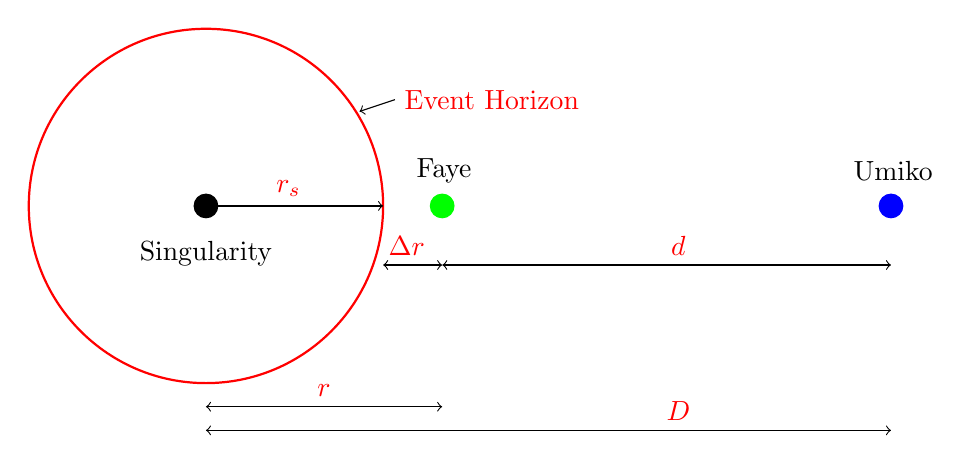
\begin{tikzpicture}[scale=1.5]
      
            % Black Hole Center (Singularity)
            \filldraw[black] (0,0) circle (0.1);
            \node at (0, -0.4) {Singularity};
      
            % Event Horizon (rs)
            \draw[thick, red] (0,0) circle (1.5);
            \node[anchor=south, red] at (0.7, 0) {$r_s$};
            \node[anchor=west, red] at (1.6, 0.9) {Event Horizon};
            \draw[<-] (1.3, 0.8) -- (1.6, 0.9);
            % Faye (near Event Horizon)
            \filldraw[green] (2, 0) circle (0.1);
            \node[anchor=west] at (1.7, 0.3) {Faye};
      
            % Umiko (at Infinity)
            \filldraw[blue] (5.8, 0) circle (0.1);
            \node[anchor=west] at (5.4, 0.3) {Umiko};
      
            % Radius (rs) Label
            \draw[<->] (0, 0) -- (1.5, 0);
            \draw[<->] (1.5,-0.5) -- (2, -0.5);
            \node[anchor=south, red] at (1.7, -0.5) {$\Delta r$};
            \draw[<->] (2.001, -0.5) -- (5.8, -0.5);
            \node[anchor=south, red] at (4, -0.5) {$d$};
            \draw[<->] (0, -1.7) -- (2, -1.7);
            \node[anchor=south, red] at (1., -1.7) {$r$};

            \draw[<->] (0, -1.9) -- (5.8, -1.9);
            \node[anchor=south, red] at (4, -1.9) {$D$};

            % Labels
            % \node[anchor=west] at (0, -2) {$r_s$: s, $r$: radial distance};
            
      
          \end{tikzpicture}
        }
        \caption{Schwarzschild Black Hole Diagram ($Faye$: Observer Near the BH, $Umiko$: Observer far from the BH, $r_s$: Schwarzchild radius, $\Delta r$: Distance of Faye from the Event Horizon, $r$: radial distance, $d$: distance of Umiko from Faye, $D$: distance of Umiko from Singularity)}
        \label{fig:blackhole}
  
      \end{figure*}


      In case of Umiko, as she is too far from the black hole, (infinity if we talk in gravitational field terms), instead of having a constant distance value for her, we set a constant acceleration due to the gravity (several thousands times less than \(g_e\)) she will experience and calculated her distance \((D)\) from the black hole and then her distance \((d)\) to Umiko. This allowed us to change mass of the BH without having to worry about the relativistic effects. 

      For distance \(D\) calculation we rearranged the ``Newtonian Gravitational acceleration'' equation as for thousands of times low value of \(g_e\) is weak enough gravity for Newtonian equations to be valid.

      \begin{equation}
        \boxed{D = \sqrt{\frac{GM}{a}}}
      \end{equation}

      \begin{info}
        For Umiko, far out from the gravitational well of BH, coordinate quantities and proper ones are both same, as \(r\) for her will be so large, making term \(q\) for her negligible. Also, why Newtonian equations are valid for her.
      \end{info}

      Using \(D\) and subtracting \(r\), Faye's distance from the Singularity, we can get the distance from Faye to Umiko. This will also be the distance that the signal between them will be travelling, given by, 

      \begin{equation}
        \boxed{d = D - r}
      \end{equation}

      \subsection{Time}

      Umiko's clock far from the BH, will run smoothly, i.e. at normal rate, and measure time that will be same as her coordinate time \(t\). Faye on the other hand will experience extreme time dilation, i.e. her single second could be hours or days for Umiko depending on how far Faye is from the black hole. To get the sense of Faye's \textbf{``Proper Time''} \((\tau)\), given by, 
      
      \begin{equation} \label{eq: tau1}
        \boxed{\tau = t q}
      \end{equation}

      where, \(q\) is from equation (ref), we will set \(\tau\) as \(1 \) \(second\) and see how many seconds will pass for Umiko. This will simply be equal to the inverse of \(q\) as can be seen by,

      \begin{equation}
        \boxed{t = \tau \cdot \frac{1}{q}}
      \end{equation}

      putting \(\tau = 1\) second, we get, 

      \begin{equation}
        \boxed{t = \frac{1}{q}}
      \end{equation}


    \subsection{Signal}

    Now, with \emph{Mass, Distances and Time} all defined, we are ready to go into the mode of the conversation between Faye and Umiko, \emph{Morse code}. As mentioned in the start, the dots and dashes will be differentiated based on the duration of the signal, that will be emitted by the signal torch. However, like with time and distance, the light and it's properties like, wavelength will be effected as it travel to and from the BH gravitational field. 

    In simple, any light travelling towards the black hole gets redder, i.e. it's wavelength increases and it streches out and loses energy, causing \textbf{gravitational redshift}, while in the opposite scenario, lights gain energy and it's wavelength decreases. Interesting thing is that the gain or loss, in both cases is defined by the same factor and it's inverse, aka \textbf{``gravitational redshift''} \((z)\), given by in terms of \(q\) as, 

    \begin{equation}
        \boxed{z = -1 + \frac{1}{q}}
    \end{equation}

    which then can be used to calculate the wavelength \((\lambda_o)\) as it is observed by the observer near the event horizon, as a function of emitted wavelength \((\lambda_e)\) and gravitational redshift \((z)\), 

    \begin{equation}
        \boxed{\lambda_o = \lambda_e (1 + z)}
    \end{equation}

    It is also clear from the above equation that the observed wavelength \(\lambda_o\) will be \(1 + z\) times greater than \(\lambda_e\), meaning, it will be redshifted.

    On the other side, for Umiko, the light will be blue shifted with the inverse of the same factor \(1 + z\), given by, 

    \begin{equation}
        \boxed{\lambda_{o}' = \lambda_{e}' \cdot \frac{1}{(1+z)}}
    \end{equation}

    For our purposes, instead of defining the emitted wavelength, we will set a fixed observed wavelength for both of them and rearrange the equations to figure out the wavelengths that their signal torches will be using.

    As stated earlier, clocks of both Faye and Umiko will run at different rate, however, we want the length of flash to be same for both of them, i.e. like for both of them the dot flash will always be, say \(3\) seconds long, \((t_{\cdot)}\). This means that both of them would have to emit the signal for longer (in Umiko's case) or much shorter (Faye's case), in order for the other person to observe it as \(3\) seconds, just like with the wavelength of the signal. 

    In order to find the time the will emit their respective signal to get the desired length observed by the other person, we will use the equation for time dilation. For Faye emitted signal length, her proper time will be calculated in terms of coordinate time \(t\) as \((t_{\cdot})\) length and for Umiko her coordinate time will be calculated for by putting \((t_{\cdot})\) length in terms of proper time \(\tau\).
    
    Further more, message duration can be calculated as the sum of the dot \((t_{\cdot})\) and dash \((t_{-})\) length in a message, multiplied with the number of dots \((n)\) and dashes \((m)\) respectively as given in, 
    
    \begin{equation}
      \boxed{t_s = n(t_{\cdot}) + m(t_{-})}
    \end{equation}

    and then the Signal travel time (T) can be calculated using, 

    \begin{equation}
      \boxed{T = \frac{d}{c}}
    \end{equation}
    

    \begin{info}
      \textbf{G-Forces for Faye:} In order for Faye to hover at a distance \(\Delta r\) from the event horizon of the black hole, she will experience the g-forces, or acceleration (relativistic), which can be calculated using, 

      \begin{equation}
        \boxed{g = \frac{GM}{r^2} \cdot\frac{1}{q}}
      \end{equation}
    \end{info}
  \section{Values to the Parameters}

  Now, equipped with the tools of equations, we are finally ready to have some quantitative insight into the conversation between Faye and Umiko. So, let's summarise which parameters are predefined by us and which will be derived based on the predefined ones.

  \begin{description}
    \item[predefined ->] derived \\-> derived from the derived
    \item[Tidal acceleration \((a_t)\) ->] Mass \((M)\) of SBH \\-> Schwarzchild radius \((r_s)\)
    \item[Proper Distance \((\Delta r')\) ->]  Coordinate distance (Faye) \((\Delta r)\) \\-> Radial Distance \(r\)  \\-> \(q\) \\-> Gravitational redshift \((z)\)
    \item[Proper Time \((\tau)\) ->] Coordinate time (\(t\))
    \item[Accelaration (Umiko) \((a)\) ->] Distance from Umiko to Singularity \((D)\) \\-> distance from Umiko to Faye \((d)\) \\-> Signal travel time \((T)\)
    \item[Observed wavelength \((\lambda_o)\) \& \((\lambda_{o}')\)] ->  Emitted wavelength \((\lambda_{e})\) \& \((\lambda_{e}')\)
    \item[Dot-Dash lengths \((t_{\cdot})\) \& \((t_{-})\) ->]  Signal Duration \((t_s)\) 
  \end{description}

  So let's assign them Values

  \begin{table}[H]
    \centering
    \caption{Data Values}
    \label{tab:table}
    \begin{tabular}{ll}
        \toprule
        \textbf{Parameter} & \textbf{Value} \\
        \midrule
        Tidal acceleration \((a_t)\) & \(g_e\) or \(9.8 ms^2\) \\
        Proper Distance \((\Delta r')\) & \(10\) meters \\
        Proper Time \((\tau)\) & \(1\) second \\
        Umiko's Acceleration \((a)\) & \(g_e / 10^{6}\) \\
        Faye's Observed wavelength \((\lambda_{o}')\) & \(690 \times 10^{-9}\) meters \\
        Umiko's Observed wavelength \((\lambda_{o})\) &  \(470 \times 10^{-9}\) meters\\
        Dot length \((t_{\cdot})\) & \(3\) seconds\\
        Dash length \((t_{-})\) & \(7\) seconds \\

        \bottomrule   
    \end{tabular}

    \tabletext{Note: All these values can be changed}

\end{table}

Then we used the following python script to calculate the rest of the quantities. 

\begin{table}[H]
  \centering
  \caption{Data Values}
  \label{tab:table}
  \begin{tabular}{ll}
      \toprule
      \textbf{Parameter} & \textbf{Value} \\
      \midrule
      Mass \((M)\) & \(45843.223\) \(M_{\odot}\)\\
      Schwarzchild radius \((r_s)\) & \(1.353 \times 10^{8}\) m\\
      Faye's Coordinate Distance \((\Delta r)\) & \(7.450 \times 10^{-7}\) m \\
      Faye's Radial Distance \((r)\) & \(1.353 \times 10^{8}\) m \\
      q \((q)\) & \(7.450 \times 10^{-8}\)\\
      Coordinate Time \((t)\) & \(13421773\) s \\
      G-forces for Faye \((g)\) & \(4.454 \times 10^{15}\) \(ms^2\)\\
      Umiko's Distance to Singularity \((D)\) & \(7.87663 \times 10^{12}\) m \\
      Umiko's distance to Faye \((d)\) & \(7.87649 \times 10^{12}\) m \\
      Faye's emitted wavelength  \((\lambda_{e}')\) & \(3.501 \times 10^{-14}\) m \\
      Umiko's emitted wavelength  \((\lambda_{e})\) & \(12.884 \) m \\
      Signal Duration\((t_s)\) & \\
      Signal Travel Time \((T)\) & \(26272.711\) s \\
      


      \bottomrule   
  \end{tabular}

  \tabletext{Note: All these values can be changed}

\end{table}

  \newpage

  \section*{Derivations}

  \subsection*{Mass of the Black hole}

  According to \emph{Newton's 2nd law},

  \begin{equation} \label{eq: 1.1}
    F = ma \tag{1.1}
  \end{equation}

  In case, of acceleration due to gravity \((g)\), this can be written as, 

  \begin{equation} \label{eq: 1.2}
    F_g = mg \tag{1.2}
  \end{equation}
  
  And in accordance with \emph{Newton's Law of Gravitation}, 

  \begin{equation} \label{eq: 1.3}
    F_g = \frac{GMm}{r^2} \tag{1.3}
  \end{equation}

  From equation \eqref{eq: 1.2} and \eqref{eq: 1.3}, we get \(g\), Gravitational acceleration as, 

  \begin{equation} \label{eq: 1.4}
    g = \frac{GM}{r^2} \tag{1.4}
  \end{equation}

  Tidal acceleration \((a_t)\) or Gravitational gradient \((\Delta g)\) is defined as the rate of change of gravitational acceleration across small distance \(\Delta r\), given by the derivative of \(g\) from equation \eqref{eq: 1.4}, as

  \begin{align} \label{eq: 1.8}
     \frac{dg}{dr} &= \frac{d}{dr} (\frac{GM}{r^2}) \tag{1.5}\\
     \frac{dg}{dr} &= GM\frac{d}{dr} (r^{-2}) \tag{1.6}\\
     \frac{dg}{dr} &= GM (2 r^{-3}) \tag{1.7}\\
     \frac{dg}{dr} &= \frac{2GM}{r^{3}} \tag{1.8}
  \end{align}
  
 For a finite change in r as \(\Delta r\), for a finite change in g, \(\Delta g\),

  \begin{equation} \label{eq: 1.9}
    \Delta g = \frac{dg}{dr} \Delta r \tag{1.9}
  \end{equation}
 
  from equation \eqref{eq: 1.9} and \eqref{eq: 1.8}, and replacing \(Delta r\) with \(h\) to represent height of a person, we get the same equation as in \eqref{eq:tidal acceleration}, 

  \begin{equation} \label{eq: 1.10}
    \Delta g = \frac{2GMh}{r^{3}} \tag{1.10}
  \end{equation}

  Till here, the derivation can be found in text books. Afterwards, we are gonna solve it for our purposes. 

  We would like to derive an equation that calculate the mass of the BH \(M\), that has a certain \(\Delta g\) at the surface of it's event horizon, i.e.~at \(r_s\). 

  \begin{note}
    We used \(r_s\) instead of radial distance \(r\), because it leads to the equation of kind \((a+b)^3\), which then ends up turning cubic as well as squared multiple terms for \(r_s\), which we are trying to eliminate.
  \end{note}

  As, \(r_s = 2GM/c^2 \) and putting \(r = r_s\) in equation \eqref{eq: 1.10}, we get, 

  \begin{align} \label{eq: 1.16}
    \Delta g &= 2GMh (\frac{c^2}{2GM})^3 \tag{1.11} \\
    \Delta g &= 2GMh \frac{c^8}{8G^3 M^3} \tag{1.12} \\
    \Delta g &= h \frac{c^8}{4G^2 M^2} \tag{1.13} \\
     M^2 &=  \frac{hc^8}{4G^2 \Delta g} \tag{1.14} \\
     M &= \sqrt{\frac{hc^8}{4G^2 \Delta g} \tag{1.15}} \\
     M &= \frac{c^3}{2G}\sqrt{\frac{h}{\Delta g} \tag{1.16}}  
  \end{align}

  where, \eqref{eq: 1.16} is the desired equation \eqref{eq: mass_at}.
  
  \begin{info}
    From equation \eqref{eq: 1.16}, separating constants, and \(h\), we get the relation

    \begin{equation*}
      M \propto \frac{1}{\sqrt{\Delta g}}
    \end{equation*}
    
    which implies that the more massive a Black Hole, the weaker are tidal forces, aka gravitational gradient at it's event horizon. 
  \end{info}

  \subsection*{Proper and Coordinate Distances}

  The \emph{Schwarzchild Metric} is given by, 

  \begin{equation} \label{eq: Sm}
    ds^2 = -c^2d\tau^2 = -(1 - \frac{r_s}{r}) c^2 dt^2 + (1 - \frac{r_s}{r})^{-1} dr^2 + r^2 (d\theta^2 - sin^2\theta d\phi^2) \tag{2.1}
  \end{equation}

  where \((t, r, \theta, \phi)\) are \emph{Schwarzchild coordinates} that describe the curvature around a non-rotating, uncharged spherical body (black hole). 
  
  for simplification of the equation to get the relation for proper and coordinate distance, we will assume a spacetime event that is fixed in time, \(dt = 0\), and no angular motion, i.e. a pure radial movement, hence, \(d\theta = d\phi = 0\), which simplifies equation \eqref{eq: Sm} to, 

  \begin{equation} \label{eq: 2.2}
    ds^2 = (1 - \frac{r_s}{r})^{-1} dr^2 \tag{2.2}
  \end{equation}
  then for a proper distance \((\Delta r')\) for coordinate distance \((\Delta r)\), we have, 
  
  \begin{align*} \label{eq:2.3}
    \Delta r' &= \sqrt{ds^2}  \\
    \Delta r' &= \sqrt{(1- \frac{r_s}{r})^{-1} \Delta r^2}  \\
    \Delta r' &= \Delta r \sqrt{(1 - \frac{r_s}{r})^{-1}} \\
    \Delta r' &= \Delta r \frac{1}{\sqrt{1- \frac{r_s}{r}}} \tag{2.3} 
  \end{align*}

  where , substituting \(\sqrt{1 - (rs/r)}\) as \(q\) will gives us equation \eqref{eq: qr}. 

  Now, Further more, 

  \begin{align*} \label{eq: 2.4}
    \Delta r &= \Delta r' \sqrt{1- \frac{r_s}{r}} \\
    \Delta r &= \Delta r' \sqrt{\frac{r - r_s}{r}} \\
    \Delta r &= \Delta r' \sqrt{\frac{r_s + \Delta r - r_s}{ r_s + \Delta r}} \text{    from eq \eqref{eq: r}} \\
    \Delta r &= \Delta r' \sqrt{\frac{ \Delta r }{ r_s + \Delta r}} \\
    \Delta r^2 &= \Delta r'^2 \frac{\Delta r }{ r_s + \Delta r} \\
    0 &= \Delta r^2 (r_s + \Delta r) - \Delta r'^{2} \Delta r \\
    0 &= \Delta r^3 + r_s\Delta r^2 - \Delta r'^{2} \Delta r \\
    0 &= \Delta r(\Delta r^2 + r_s\Delta r - \Delta r'^{2})  \tag{2.4}
  \end{align*}
  
  from equation \eqref{eq: 2.4}, we get \(\Delta r = 0\) and the quadratic equation, 

  \begin{equation*} \label{eq: 2.5}
    \Delta r^2 + r_s\Delta r - \Delta r'^{2} = 0 \tag{2.5}\
  \end{equation*}

  comparing with the general quadratic equation, \(ax^2 + bx + c = 0\), we get, 
  \begin{align*}
    a &= 1 \\
    b &= r_s \\ 
    c &= -\Delta r'
  \end{align*}

  using quadratic formula \eqref{eq: QF}, 

  \begin{equation} \label{eq: QF}
    x = \frac{-b \pm \sqrt{b^2 - 4ac}}{2a} \tag{QF}
  \end{equation}

  putting values we get, 

  \begin{equation} \label{eq: dr}
    \Delta r = \frac{-r_s \pm \sqrt{r_s^2 + 4(\Delta r')r_s}}{2} \tag{2.6}
  \end{equation}

  \subsection*{Proper and coordinate Time}

  For a timelike spacetime event, we will assume an event that is stationary in space, i.e. \(ds = d\theta = d\phi = 0\), which reduces the \emph{Schwarzchild Metric} to,

  \begin{equation} \label{eq: pt}
    -c^2d\tau^{2} = - (1 - \frac{r_s}{r}) c^2 dt^2 \tag{2.7}
  \end{equation}

  simplifying it by cancelling out \(-c^2\) on both sides, and taking the square root and neglecting the derivative, leaves the following, 

  \begin{equation} \label{eq: pt2}
    \tau = t \cdot \sqrt{1 - \frac{r_s}{r}} \tag{2.8}
  \end{equation}
  or, using equation \eqref{eq: q}, we get the same equation as \eqref{eq: tau1}

  \begin{equation} \label{eq:Tau2}
    \tau = tq \tag{2.9}
  \end{equation}

  \subsection*{Gravitational redshift}

  to be written...

  \section*{Model}

  \begin{figure}[H]
    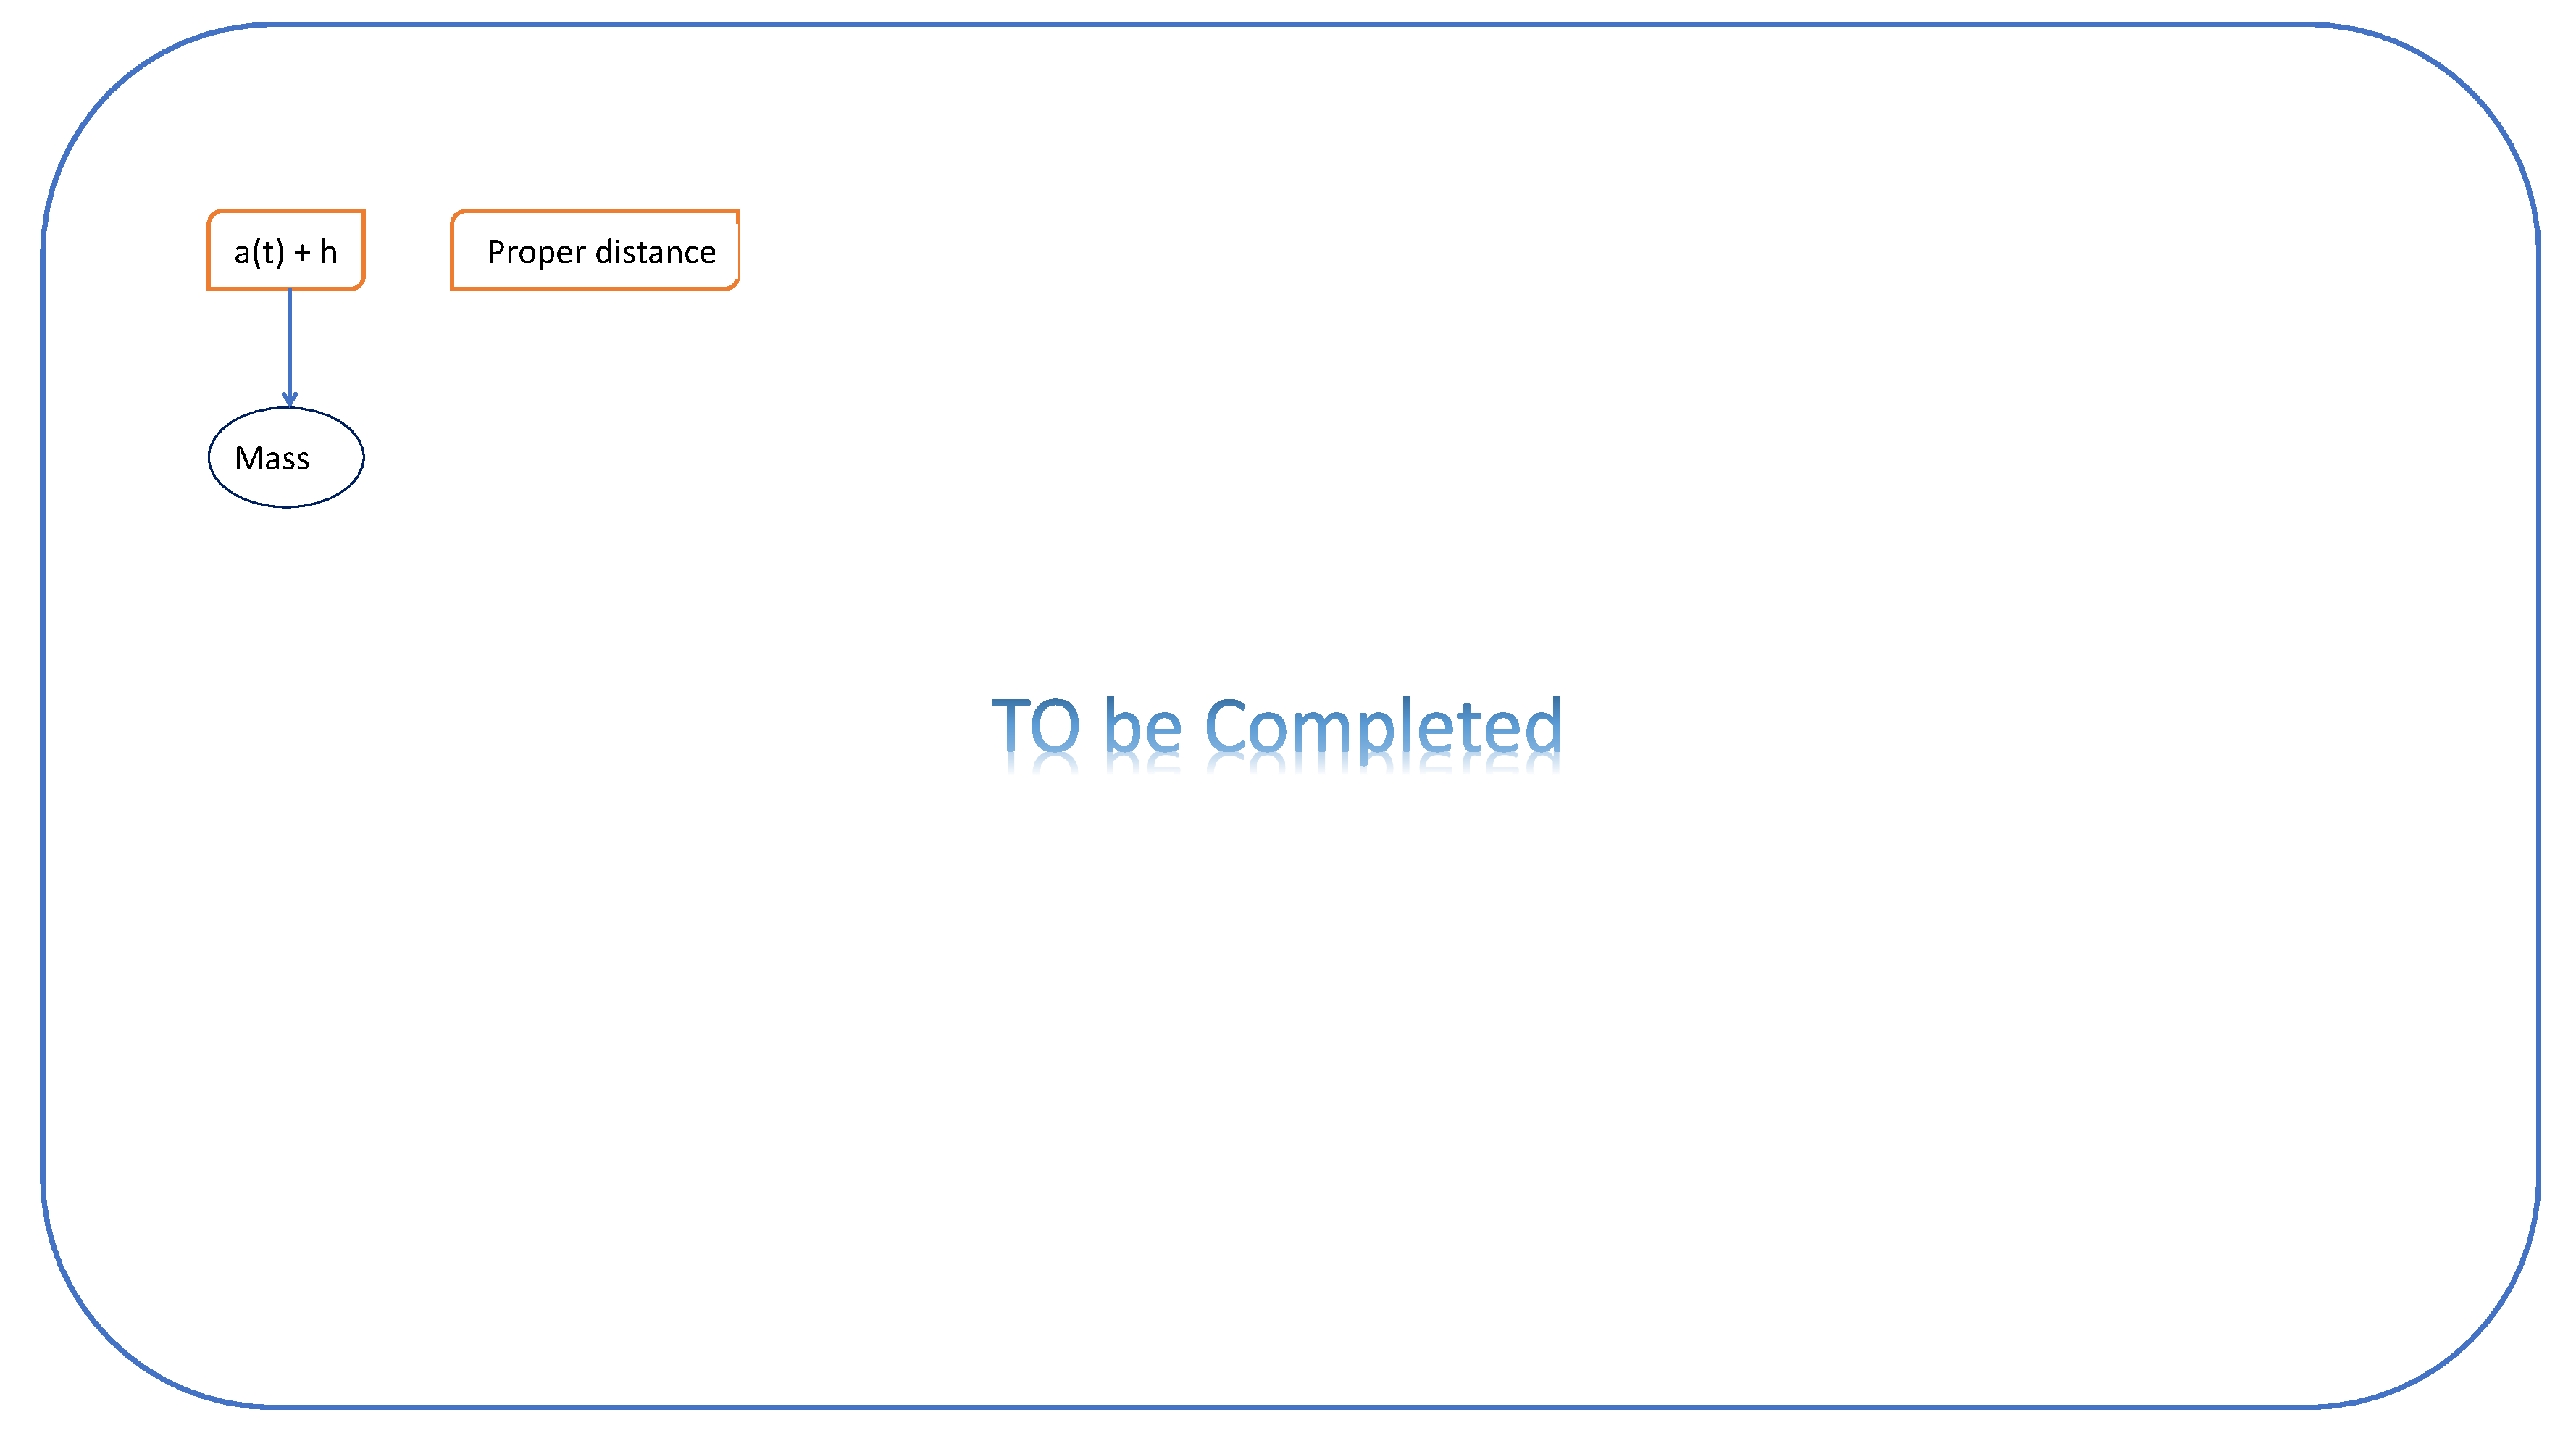
\includegraphics[width=\linewidth]{model.pdf}
  \end{figure}
  
  \section*{Remaining stuff}

  following things remain to get this phase, settled, 

  \begin{itemize}
    \item A page of definations, (appendix 1)
    \item A list of constants and symbols (appendix 2)
    \item Some reviewing text and rewritting
    \item some derivations and formula checking
    \item the proper model for all of it 
    \item morse code script and message settings etc. 
    \item script (python class code for the model)
    \item the next step, is adding info and formulas figuring out for rates of changes in parameters and how things change.
    \item then turning it all into useable website
    \item a summarised story
  \end{itemize}

  this should give you some idea what we are doing, which is doing as we please. Instead of doing things classically, that is to choose one specific goal, research it and then mix things up or use new data to get something new. We are following an idea, a sort of thought experiment, which keeps on redefining as we move on to it. It's fine. And obviously the final thesis will not be in this format. There's a lot but i'll leave it here and take a break. Then start things off from a different perspective. Don't worry and if you have any queries. You know where to find me. (this is the work of less than few days. most time was spend into to setting the formulas straight and redefining them to our set up and that was the most fun part of it. also formulas need to be checked by a physics or maths specialist but there are few of them remainings so i'll get them checked once i have most of them straightened out, proably by the end of next week)
\end{document}
